\documentclass[../../main/main.tex]{subfiles}
\graphicspath{{./figures/}}

\makeatletter
\renewcommand{\@chapapp}{Optique -- chapitre}
\makeatother

% \toggletrue{student}
% \HideSolutionstrue

\begin{document}
\setcounter{chapter}{3}

\chapter{\switch{Correction du TD}{TD~: Dispositifs optiques}}

\section{Vergence et grandissement de lentilles accolées}
\switch{
	Soit le système de deux lentilles $\Lc_1$ et $\Lc_2$, de centres optiques
	$O_1$ et $O_2$ et de vergences $V_1$ et $V_2$ qui sont \textit{accolées}
	(c'est-à-dire de même axe optique et de centres optiques confondus~: dans la
	pratique, on veut $|\obar{O_1O_2}| \ll |f_1'|$ et $\ll |f_2'|$ simultanément).

	\begin{enumerate}
		\item Montrer qu'il est équivalent à une lentille $\Lc$ de vergence $V = V_1
			      + V_2$.
		\item Préciser le grandissement de l'ensemble en fonction du grandissement
		      de chaque lentille.
	\end{enumerate}
}{
	\begin{enumerate}
		\item Dans cette situation, on a le système $\rm A \opto{\Lc_1}{\rm O_1} A_1
			      \opto{\Lc_2}{O_2} A'$, avec $\rm O_1 = O_2 = O$. Une lentille équivalente à ce
		      système ferait passer directement de A à A' et aurait une distance
		      focale $\OFp$ telle que
		      \begin{equation}\label{eq:vaccol}
			      \frac{1}{\OFp} = \frac{1}{\OAp} - \frac{1}{\OA}
		      \end{equation}
		      Pour faire apparaître les vergences des lentilles une et deux, on
		      peut~:
		      \begin{enumerate}
			      \item Écrire les relations de conjugaison pour les deux lentilles~:
			            \begin{equation*}
				            \boxed{\frac{1}{\obar{\rm OF'_1}} =
					            \frac{1}{\obar{\rm OA_1}} -
					            \frac{1}{\OA}}
				            \qet
				            \boxed{\frac{1}{\obar{\rm OF'_2}} =
					            \frac{1}{\OAp} -
					            \frac{1}{\obar{\rm OA_1}}}
			            \end{equation*}

			      \item Ou directement dans~\ref{eq:vaccol} ajouter et retirer
			            $\frac{1}{\obar{\rm OA_1}}$ dans le terme de droite.
		      \end{enumerate}
		      Quoiqu'il en soit, on trouve rapidement
		      \begin{align*}
			      \frac{1}{\OFp} & =
			      \frac{1}{\obar{\rm OF'_1}} + \frac{1}{\obar{\rm OF'_2}}
			      \\\Leftrightarrow
			      V              & = V_1 + V_2
		      \end{align*}
		\item Le grandissement de l'ensemble est $\gamma =
			      \dfrac{\OAp}{\OA}$. Or, $\gamma_1 =
			      \dfrac{\obar{\rm OA_1}}{\OA}$ et
		      $\gamma_2 = \dfrac{\OAp}{\obar{\rm OA_1}}$~; on a donc
		      \begin{empheq}[box=\fbox]{equation*}
			      \gamma = \gamma_1\gamma_2
		      \end{empheq}
	\end{enumerate}
	\begin{tcb}[label=rema:prod_gamma](rema){Produit des grandissements}
		Si le théorème des vergences (c'est son nom) ne vaut que pour des lentilles
		accolées (une version plus générique s'écrit $V = V_1 + V_2 -
			\obar{O_1O_2}V_1V_2$), l'expression du grandissement \textbf{vaut pour toute
			association}.
	\end{tcb}
}

\section{L'œil hypermétrope et sa correction}

\switch{
	Dans cet exercice, on étudie un œil assimilé à une lentille mince convergente
	$\Lc$, dont le centre optique $S$ se trouve à une distance constante $d =
		\SI{17}{mm}$ de la rétine. Cet œil est hypermétrope et donne d'un objet à
	l'infini une image située \SI{1.5}{mm} derrière la rétine lorsqu'il est au repos.

	\begin{enumerate}
		\item Déterminer la distance focale de cet œil au repos. On la considèrera
		      constante dans la suite du problème, l'œil n'accommodant pas.
		\item L'œil est-il trop ou pas assez convergent ? Corrige-t-on ce défaut en
		      ajoutant des verres de lunettes convergents ou divergents ?
		\item L'œil est corrigé par un verre de lunettes, assimilé à une lentille
		      mince de centre optique $O$ et
		      placé à une distance $d = \SI{12}{mm}$ du centre optique $S$ de l'œil
		      réduit. On souhaite que dans ces conditions, l'œil au repos ait une
		      vision nette d'un objet situé à l'infini.
		      \begin{enumerate}
			      \item tooleler l'endroit où doit se trouver l'image définitive
			            donnée par l'œil corrigé.
			      \item Quels points caractéristiques du verre et de l'œil doivent
			            être confondus afin de corriger la vision de loin ?
			      \item Déterminer la distance focale puis la vergence du verre
			            correcteur.
			      \item Faire un schéma de principe expliquant la correction de l'œil
			            par les lunettes.
		      \end{enumerate}
	\end{enumerate}
}{
	\begin{center}
		\begin{tcb}[sidebyside](data){Données}
			\begin{itemize}
				\item Œil = lentille $(\Lc, \rm S)$ ;
				\item $\obar{\rm SE} = \SI{17}{mm}$ ;
				\item $\obar{\rm SA} = -\infty \Rightarrow \obar{\rm SA'} = \obar{\rm
						      SE} + \SI{1.5}{mm}$
			\end{itemize}
			\tcblower
			\tcbsubtitle{Schéma}
			\begin{center}
				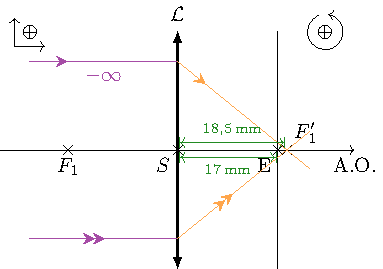
\includegraphics{oeil_hyper-data.pdf}
			\end{center}
		\end{tcb}
	\end{center}

	\begin{enumerate}
		\item ~
		      \begin{tcbraster}[raster columns=5, raster equal height=rows]
			      \begin{tcb}(ques){Résultat}
				      \[\obar{\rm SF'}\]
			      \end{tcb}
			      \begin{tcb}*[raster multicolumn=2](tool){Outil}
				      On trouve le point focal image d'un système en étudiant l'image d'un
				      objet à l'infini.
			      \end{tcb}
			      \begin{tcb}[raster multicolumn=2](appl)'r'{Application}
				      Ici, la lecture de l'énoncé donne directement la réponse~: le
				      point focal image et \SI{1.5}{mm} derrière la rétine. On a donc
				      \[\obar{\rm SF'} = \SI{18.5}{mm}\]
			      \end{tcb}
		      \end{tcbraster}
		\item L'œil n'est pas assez convergent, il faudrait que les rayons se
		      croisent plus tôt sur l'axe optique pour que l'image se forme sur la
		      rétine. Il faut donc corriger avec des lentilles correctrices
		      convergentes.

		\item ~
		      \begin{center}
			      \begin{tcb}[sidebyside](data){Données}
				      \begin{itemize}
					      \item Verre lunette = $(\Lc_v, \rm O)$ ;
					      \item $\obar{\rm OS} = \SI{12}{mm}$ ;
					      \item $\AB \opto{\Lc_v}{\rm O} \ABb \opto{\Lc}{\rm S} \ABp$
				      \end{itemize}
				      \tcblower
				      \tcbsubtitle{Schéma}
				      \begin{center}
					      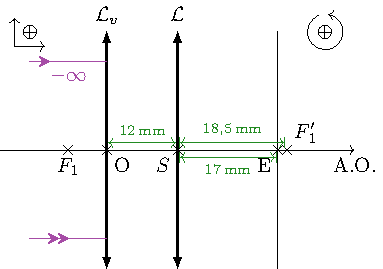
\includegraphics{oeil_hyper-verre.pdf}
				      \end{center}
			      \end{tcb}
		      \end{center}
		      \begin{enumerate}
			      \item ~
			            \begin{center}
				            \begin{tcb}[width=.5\linewidth](rapp){Rappel}
					            L'image doit se former sur l'écran de la lentille,
					            autrement dit la rétine~: avec $\AB = -\infty$ on doit
					            avoir $\rm A' = E$.
				            \end{tcb}
			            \end{center}
			      \item ~
			            \begin{tcbraster}[raster equal height=rows]
				            \begin{tcb}(ques){Résultat attendu}

					            Utiliser le fonctionnement physique du système pour
					            déterminer comment associer la lunette à l'œil.

				            \end{tcb}
				            \begin{tcb}(appl)'r'{Application}
					            \begin{center}
						            \begin{tikzpicture}[]
							            \node[] (AB) at (0,0) {$\AB$};
							            \node[] (A_1B_1) at (2,0) {$\ABb$};
							            \node[] (A'B') at (4,0) {$\ABp$};
							            \draw[->] (AB) -- (A_1B_1)
							            node [midway, above] {$\Lc_v$}
							            node [midway, below] {O};
							            \draw[->] (A_1B_1) -- (A'B')
							            node [midway, above] {$\Lc$}
							            node [midway, below] {S};
							            \node[below=0.3, Purple!70]
							            (AB) at (AB) {$-\infty$};
							            \node[below=0.3, brandeisblue]
							            (A1B1b) at (A_1B_1) {$A_1 = F'_v$};
							            \node[below=0.3, ForestGreen]
							            (A1B1bb) at (A1B1b) {$A_1 = R$};
							            \node[below=0.3, orange!70]
							            (A'B'b) at (A'B') {$A' = E$};
							            \draw[->, Purple!70]
							            (AB) to[bend right] (A1B1b.west);
							            \draw[->, orange!70]
							            (A'B'b) to[bend left] (A1B1bb.east);
						            \end{tikzpicture}
					            \end{center}
					            On a donc $\rm A_1 = F'_v = R$.
				            \end{tcb}
			            \end{tcbraster}
			            \begin{tcb}(ror){Important !}

				            Attention, \textbf{seul} le remotum de l'œil emmétrope
				            est à l'infini. Vérifiez bien vos définitions.

			            \end{tcb}
			      \item ~
			            \begin{tcbraster}[raster columns=2, raster equal height=rows]
				            \begin{tcb}(ques){Résultats attendus}

					            On cherche $\obar{\rm OF'_v}$ sachant que $\rm F'_v = R$~:
					            l'idée est donc de trouver R de l'œil connaissant sa
					            distance focale et la distance œil-écran.

				            \end{tcb}
				            \begin{tcb}(tool)'r'{Outil}

					            On va donc utiliser la formule de conjugaison d'une
					            lentille mince~:

					            \[ \frac{1}{\OFp} = \frac{1}{\OAp} - \frac{1}{\OA}\]
				            \end{tcb}
			            \end{tcbraster}
			            \begin{center}
				            \begin{tcb}(appl){Application}
					            Avec les données de l'exercice, on a

					            \[
						            \frac{1}{\obar{\rm SF'}} =
						            \frac{1}{\obar{\rm SE}} -
						            \frac{1}{\obar{\rm SR}}
					            \]
					            Soit
					            \begin{equation*}
						            \boxed{
							            \obar{\rm SR} =
							            \frac{
								            \obar{\rm SE}\obar{\rm SF'}}{
								            \obar{\rm SF'}-\obar{\rm SE}}
						            }
						            \quad \text{avec}\quad
						            \left\{
						            \begin{array}{rcl}
							            \obar{\rm SE}  & = & \SI{17}{mm}   \\
							            \obar{\rm SF'} & = & \SI{18.5}{mm}
						            \end{array}
						            \right.
					            \end{equation*}
					            Et
					            \[
						            \boxed{\obar{\rm SR} = \SI{21}{cm}}
					            \]
					            Avec la composition des distances et comme $\rm F'_v = R$,
					            on a finalement
					            \[
						            \boxed{
							            \obar{\rm OF'_v} =
							            \obar{\rm OS} + \obar{\rm SR} =
							            \num{1.2}+\num{20.9} = \SI{22}{cm}}
					            \]
					            Soit \fbox{$V_{\rm verre} = \SI{+4.5}{\de}$}
				            \end{tcb}
			            \end{center}
			      \item On a donc
			            \begin{center}
				            \hspace*{-2cm}
				            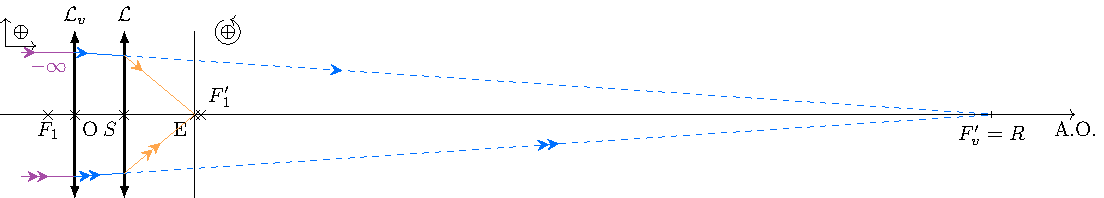
\includegraphics{oeil_hyper-fin}
			            \end{center}
		      \end{enumerate}
	\end{enumerate}
}

\section{Élargissement d'un faisceau laser}
\switch{
	Un laser est un faisceau lumineux cylindrique dont le diamètre est de l'ordre
	du millimètre. Comment procéder pour élargir ce faisceau jusqu'à lui donner un
	diamètre de quelque centimètres, en utilisant une lentille divergente et une
	lentille convergente~?
}{
	\begin{minipage}{0.65\linewidth}
		On peut associer deux lentilles, la première divergente de très courte
		focale $f'_1$ ($< 0$) et la seconde convergente de grande focale $f'_2$, à
		condition de faire coïncider le foyer image $F'_1$ de la première avec le
		foyer objet $F_2$ de la seconde. Si $D$ est le diamètre du faisceau final et
		$d$ celui du faisceau initial, alors en utilisant le théorème de Thalès
		$D/f'_2 = -d/f'_1$~; pour $d = \SI{2}{mm}$ et $D = \SI{3}{cm}$, il nous faut
		\begin{empheq}[box=\fbox]{equation*} f'_2 = -15 f'_1
		\end{empheq}
	\end{minipage}
	\hfill
	\begin{minipage}{0.30\linewidth}
		\begin{center}
			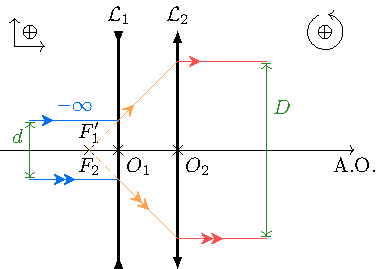
\includegraphics[width=\linewidth]{laser_elarg.pdf}
		\end{center}
	\end{minipage}
}

\section{Étude d'un photocopieur}

\switch{
	\begin{minipage}{0.55\linewidth}
		Un photocopieur permet la formation de l'image d'un document sur une surface
		photosensible par l'intermédiaire d'un objectif de reproduction. On désire
		reproduire un document de format A4 soit en A4 (même format), soit en A3
		(format double en surface) soit en A5 (format moitié en surface).

		On réalise ces différents tirages à l'aide d'un objectif en modifiant la
		position respective des lentilles à l'intérieur du système. La distance
		entre le document et le récepteur photosensible est de \SI{384}{mm} et l'on
		positionne une première lentille mince divergente $\Lc_1$ de distance focale
		image $f'_1 = \SI{-90}{mm}$ à \SI{180}{mm} du récepteur (figure ci-contre).
	\end{minipage}
	\begin{minipage}{0.45\linewidth}
		\begin{center}
			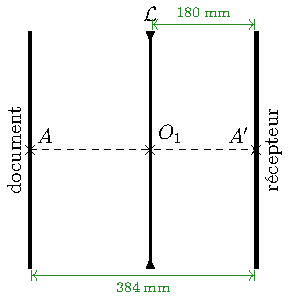
\includegraphics[width=.8\linewidth]{photocopieur-a}
		\end{center}
	\end{minipage}

	\begin{minipage}{0.55\linewidth}
		\begin{enumerate}
			\item La lentille $\Lc_1$ peut-elle donner une image du document sur le
			      récepteur ?
			\item On ajoute une lentille mince $\Lc'$ devant la lentille $\Lc_1$, à
			      \SI{180}{mm} du document (voir la figure ci-contre). La lentille
			      $\Lc'$ peut-elle être divergente ? Justifier votre réponse.
			\item Calculer la distance focale image $f'$ de cette lentille $\Lc'$
			      pour obtenir une image réelle du document sur le récepteur. Pour
			      cela, on utilisera deux relations de Descartes.
			\item En déduire le grandissement $\gamma$ de l'association des deux
			      lentilles et indiquer quel type de tirage permettra cet objectif :
			      transformer du A4 en A3 ou du A4 en A5 ?
		\end{enumerate}
	\end{minipage}
	\begin{minipage}{0.45\linewidth}
		\begin{center}
			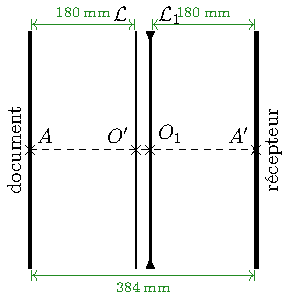
\includegraphics[width=\linewidth]{photocopieur-b}
		\end{center}
	\end{minipage}
}{
	\begin{enumerate}
		\item La lentille divergente ne peut pas donner une image réelle si l'objet
		      est réel (vérifiez avec la relation de conjugaison). Par conséquent,
		      l'image à travers $\Lc_1$ \textbf{ne peut pas être sur le récepteur},
		      car cette dernière est virtuelle.

		\item Si $\Lc'$ est divergente, l'image de A est virtuelle, comme vu
		      précédemment~; mais ça sera donc un objet réel pour $\Lc_1$, et on a
		      encore le même raisonnement. Ainsi, si une lentille peut fonctionner
		      dans ce système, elle ne peut être divergente.

		\item L'image finale est telle que $\obar{\rm O_1A'} = \SI{180}{mm}$, l'objet
		      initial est tel que $\obar{\rm O'A} = \SI{-180}{mm}$ et on a
		      $\obar{\rm O'O_1} = \SI{24}{mm}$. Avec le système $\rm A
			      \opto{\Lc'}{\rm O'} A_1 \opto{\Lc_1}{\rm O_1} A'$, on sait qu'on a les
		      relations
		      \begin{equation*}
			      \left\{
			      \begin{aligned}
				      \frac{1}{f'}   & = \frac{1}{\obar{\rm O'A_1}} -
				      \frac{1}{\obar{\rm O'A}}
				      \\
				      \frac{1}{f'_1} & = \frac{1}{\obar{\rm O_1A'}} -
				      \frac{1}{\obar{\rm O_1A_1}}
			      \end{aligned}
			      \right.
			      \Leftrightarrow
			      \left\{
			      \begin{aligned}
				      f'                & = \left( \frac{1}{\obar{\rm O'A_1}} -
				      \frac{1}{\obar{\rm O'A}} \right)^{-1}
				      \\
				      \obar{\rm O_1A_1} & = \left( \frac{1}{\obar{\rm O_1A'}} -
				      \frac{1}{f'_1} \right)^{-1}
			      \end{aligned}
			      \right.
			      \Leftrightarrow
			      \left\{
			      \begin{aligned}
				      f'                & =
				      \frac{\obar{\rm O'A_1}\times\obar{\rm O'A}}
				      {\obar{\rm O'A}-\obar{\rm O'A_1}}
				      \\
				      \obar{\rm O_1A_1} & = \frac{f'_1\times\obar{\rm O_1A'}}
				      {f'_1-\obar{\rm O_1A'}}
			      \end{aligned}
			      \right.
		      \end{equation*}
		      On en déduit
		      $\DS\obar{\rm O'A_1} =
			      \obar{\rm O_1A_1} - \obar{\rm O_1O'} =
			      \frac{f'_1\times\obar{\rm O_1A'}}
			      {f'_1-\obar{\rm O_1A'}} - \obar{\rm O_1O'}$~; avec
		      $ \left\{
			      \begin{array}{rcl}
				      f'_1             & = & \SI{-90}{mm} \\
				      \obar{\rm O_1A'} & = & \SI{180}{mm} \\
				      \obar{\rm O_1O'} & = & \SI{-24}{mm}
			      \end{array}
			      \right.$ on a
		      \[
			      \xul{\obar{\rm O'A_1} = \SI{84}{mm}}
		      \]
		      et finalement avec $\obar{\rm O'A} = \SI{-180}{mm}$, on a également
		      \[
			      \xul{f' = \SI{57}{mm}}
		      \]
		\item $\gamma_{\rm imprim} = \gamma_{\Lc'}\gamma_{\Lc_1}$ en tant
		      qu'association de lentilles~; or $\gamma_{\Lc'} =
			      \dfrac{\obar{\rm O'A_1}}{\obar{\rm O'A}} = \num{-0.5}$,
		      et $\gamma_{\Lc_1} =
			      \dfrac{\obar{\rm O_1A'}}{\obar{\rm O_1A_1}} = 3$~: on a
		      \[
			      \xul{\gamma_{\rm imprim} = \num{-1.5}}
		      \]
		      $|\gamma_{\rm imprim}| > 1$ d'une part, mais pour savoir si on peut
		      imprimer en A3 il faut savoir si la \textit{surface} est multipliée par
		      2~; $\gamma$ est un grandissement linéique (sur une longueur). Pour la
		      surface, on calcule $\gamma_{\rm imprim}^2 = 2.25 > 2$~: on peut donc
		      transformer du A4 en A3.
	\end{enumerate}
}

\section{Le microscope}

\switch{
	Un microscope est schématisé par deux lentilles minces convergentes de même
	axe optique~: l'objectif $\Lc_1$ de centre O$_1$ et de distance focale image
	$f'_1 = \SI{5}{mm}$, et l'oculaire $\Lc_2$ de centre O$_2$ et de distance
	focale image $f'_2 = \SI{25}{mm}$. On note respectivement F'$_1$ et F$_2$ les
	foyers image de $\Lc_1$ et objet de $\Lc_2$. On appelle \textit{intervalle
		optique} et on la note $\Delta$ la distance $\obar{\rm F'_1F_2} = \SI{25}{cm}$.
	L'œil de l'observataire est placé au foyer image $F'_2$ de l'oculaire. On y
	visualise un objet étendu transverse AB avec A sur l'axe optique.

	\begin{enumerate}
		\item Où doit se situer $A$ pour que l'œil n'ait pas à accommoder~? Répondre
		      en donnant l'expression et la valeur numérique de $\obar{\rm F_1A}$.
		\item On se place dans les conditions de la question précédente. Représenter
		      le trajet de 2 rayons issus de B sur une figure horizontale respectant
		      le fait que $f'_1 < f'_2 < \Delta$.
		\item Soient $\alpha'$ l'angle algébrique sous lequel l'œil voit l'image
		      finale de AB par le microscope, et $\alpha$ l'angle algébrique sous
		      lequel il apercevrait l'objet sans microscope et à la distance
		      $\Delta$. Calculer le grossissement, et interpréter son signe.
	\end{enumerate}
}{
	\begin{enumerate}
		\item L'œil visant sans fatigue à l'infini, il faut que l'image par $\Lc_2$
		      soit à l'infini. Pour ça, l'image intermédiaire A$_1$ de A par $\Lc_1$
		      doit se situer dans le plan focal objet de $\Lc_2$. Autrement dit, on
		      doit avoir $\obar{\rm F'_1A_1} = \obar{\rm F'_1F_2}$. Ceci ce traduit
		      par la schématisation optique $\rm AB \opto{\Lc_1}{\rm O_1}
			      \underbrace{\rm A_1B_1}_{\rm A_1 = F_2}\opto{\Lc_2}{\rm O_2} +\infty$.
		      On utilise donc la relation de conjugaison pour la lentille $\Lc_1$
		      avec origine au foyer~:
		      \begin{equation*}
			      \obar{\rm FA}\obar{\rm F'A'} = -f'{}^2
		      \end{equation*}
		      et avec les notations choisies, $\obar{\rm F_1A}\obar{\rm F'_1A_1} =
			      -f'_1{}^2$. On en tire directement
		      \[
			      \boxed{\obar{\rm F_1A} = \frac{-f'_1{}^2}{\Delta}}
			      \qav
			      \left\{
			      \begin{array}{rcl}
				      f'_1   & = & \SI{5}{mm}   \\
				      \Delta & = & \SI{250}{mm}
			      \end{array}
			      \right.
			      \qso
			      \xul{\obar{\rm F_1A} = \SI{-0.1}{mm}}\]
		\item ~
		      \begin{center}
			      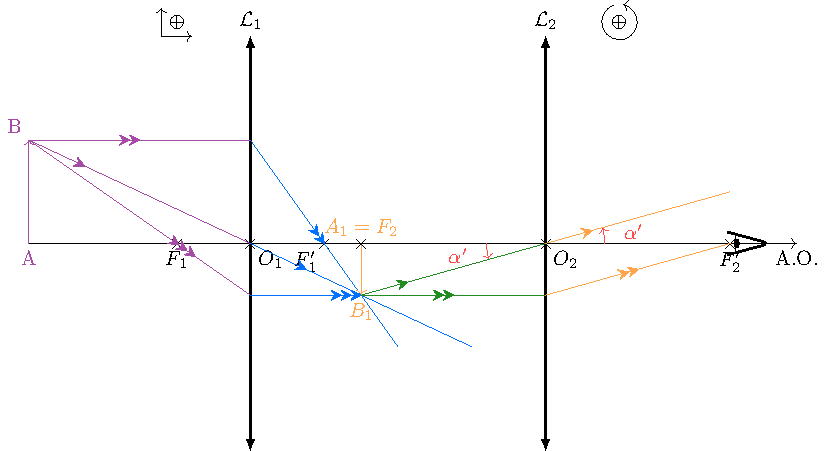
\includegraphics[width=\linewidth]{microscope.pdf}
			      \label{fig:microscope}
		      \end{center}

		\item Avec le schéma ci-dessus et dans l'hypothèse des conditions de Gauss
		      ($\tan\theta \approx \theta$), $\alpha' = \dfrac{\obar{\rm
					      A_1B_1}}{-f'_2}$. On veut relier $\obar{\rm A_1B_1}$ à $\AB$ puisqu'on
		      aura $\alpha = \dfrac{\AB}{-\Delta}$~: on utilise pour ça l'expression
		      du grandissement avec origine aux foyers (on connaît $\obar{\rm
				      F_1A}$)~:
		      \begin{gather*}
			      \gamma = \frac{\ABb}{\AB} = - \frac{\obar{\rm O_1F_1}}{\obar{\rm
					      F_1A}}
			      \\\Leftrightarrow
			      \ABb = \AB \frac{f'_1}{\obar{\rm F_1A}}
		      \end{gather*}
		      Ainsi,
		      $\DS G = \frac{\alpha'}{\alpha} =
			      \frac{
				      -\dfrac{f'_1}{f'_2} \dfrac{\AB}{\obar{\rm F_1A}}
			      }{
				      \dfrac{\AB}{-\Delta}
			      }$ donc
		      \[
			      \boxed{G = -\frac{\Delta^2}{f'_1f'_2}}
			      \qav
			      \left\{
			      \begin{array}{rcl}
				      \Delta & = & \SI{25}{cm} \\
				      f'_1   & = & \SI{5}{mm}  \\
				      f'_2   & = & \SI{25}{mm}
			      \end{array}
			      \right.
			      \qso
			      \xul{G=-500}
		      \]
	\end{enumerate}
}

\section{Lunettes astronomiques de Kepler et Galilée}

\switch{
	\subsection{Kepler}

	On construit une lunette astronomique de Kepler par un objectif $\Lc_1$ de
	diamètre $D = \SI{30}{mm}$, de centre O$_1$ et de vergence $V_1 =
		\SI{3.125}{\delta}$, et d'un oculaire $\Lc_2$ de centre $O_2$ et de vergence
	$V_2 = \SI{25}{\delta}$.

	\begin{enumerate}
		\item Calculer les distances focales images $f'_1$ et $f'_2$ de l'objectif
		      et de l'oculaire respectivement.
		\item Définir le caractère afocal d'une lunette et son intérêt pour un
		      œil emmétrope.
		\item Calculer alors l'encombrement $\obar{\rm O_1O_2}$ de la lunette.
		\item Faire un schéma à l'échelle avec comme rayons incident~:
		      \begin{itemize}
			      \item Un rayon passant par O$_1$ venant d'en haut~;
			      \item Deux rayons proches, parallèles entre eux et au premier rayon.
		      \end{itemize}
		      On prendra soin de~:
		      \begin{enumerate}
			      \item placer l'image intermédiaire donnée par l'objectif~;
			      \item puis l'image finale donnée par l'oculaire~;
			      \item tracer le cheminement du pinceau lumineux entre les deux
			            rayons proches (on hachurera la zone qu'ils délimitent).
		      \end{enumerate}
		\item Calculer le grossissement de la lunette.
		\item Rappeler la définition du cercle oculaire et son intérêt.
		\item Déterminer sa position $\obar{\rm O_2C'_K}$.
		\item Donner sa taille (diamètre $\rm D'_K$).
	\end{enumerate}

	\subsection{Galilée}

	On obtient une lunette de Galilée en remplaçant l'oculaire convergent par un
	oculaire divergent. Dans cet exercice, la valeur de la vergence est la même
	que précédemment en valeur absolue. On nomme cette lentille $\Lc_3$, son
	centre sera noté O$_3$. La lunette astronomique reste afocale.

	\begin{enumerate}
		\item Expliquer que la vergence de l'oculaire sera $V_3 = \SI{-25}{\delta}$.
		\item Calculer le nouvel encombrement $\obar{\rm O_1O_3}$.
		\item Tracer, toujours à l'échelle, le même schéma que précédemment avec
		      cette nouvelle situation.
		\item Déterminer la position $\obar{\rm O_3C'_G}$ du cercle oculaire.
		\item Donner sa taille (diamètre $\rm D'_G$).
		\item Quels sont les avantages et inconvénients de ces 2 lunettes
		      astronomiques~?
	\end{enumerate}
}{
	\subsection{Kepler}

	\begin{center}
		\begin{tcb}(data){Données}
			Association de deux lentilles~:
			\begin{enumerate}
				\item $\Lc_1$ « objectif », vergence $V_1 = \SI{3.125}{\de}$, diamètre $D
					      = \SI{30}{mm}$ ;
				\item $\Lc_2$ « oculaire », vergence $V_2 = \SI{25}{\de}$.
			\end{enumerate}
		\end{tcb}
	\end{center}

	\subsubsection{}

	\begin{tcbraster}[raster columns=7, raster equal height=rows]
		\begin{tcb}[raster multicolumn=2](ques){Résultat attendu}
			Focales de lentilles
		\end{tcb}
		\begin{tcb}*[raster multicolumn=2](tool){Outil du cours}
			\[
				V = \dfrac{1}{f'}
			\]
		\end{tcb}
		\begin{tcb}[raster multicolumn=3, valign=top](appl)'r'{Application}
			\[
				\xul{\obar{\rm O_1F'_1} = \SI{32}{cm}}
				\qet
				\xul{\obar{\rm O_2F'_2} = \SI{4}{cm}}
			\]
		\end{tcb}
	\end{tcbraster}

	\subsubsection{}
	\begin{tcbraster}[raster columns=2, raster equal height=rows]
		\begin{tcb}(data){Système afocal}
			Est afocal un système pour lequel un objet initial à l'infini donne une
			image finale à l'infini.
		\end{tcb}
		\begin{tcb}*(inte)"left"'r'{Intérêt d'un système afocal}
			Un système afocal présente comme intérêt de permettre à un œil emmétrope
			d'observer sans fatigue, étant donné que l'image sortant du système est à
			l'infini (voir cours).
		\end{tcb}
	\end{tcbraster}

	\subsubsection{}\label{sssec:k_encomb}

	\begin{tcbraster}[raster columns=7, raster equal height=rows]
		\begin{tcolorbox}[blankest, raster multicolumn=3, space to=\myspac]
			\begin{tcbraster}[raster columns=1]
				\begin{tcb}[](ques){Résultat attendu}
					$$\obar{\rm O_1O_2}$$
				\end{tcb}
				\begin{tcb}[add to natural height=\myspac](tool){Outils du cours}
					Règles de construction de rayons~:
					\begin{enumerate}
						\item Un rayon provenant de l'infini émerge d'une lentille en
						      croisant l'axe optique au plan focal image ;
						\item Des rayons se croisant dans le plan focal objet d'une lentille
						      émergent parallèles entre eux.
					\end{enumerate}
					Composition des distances~:
					\[
						\obar{\rm O_1O_2} = \obar{\rm O_1F_1'} + \obar{\rm F_1'O_2}
					\]
				\end{tcb}
			\end{tcbraster}
		\end{tcolorbox}
		\begin{tcb}[raster multicolumn=4](appl)'r'{Application}
			Pour que tous les rayons sortant de la lunette soient parallèles entre eux
			(donnant donc une image à l'infini), il faut que tous les rayons à
			l'intérieur passent par le plan focal objet de son oculaire.
			\bigbreak
			Or, tous les rayons arrivent dans la lunette parallèles entre eux (objet
			initial à l'infini) ; il se croisent donc dans le plan focal image de
			l'objectif.
			\bigbreak
			Pour que la condition soit vérifiée, il faut donc simplement que les plans
			focaux image de $\Lc_1$ et objet de $\Lc_2$ soient confondus ; autrement
			dit~:
			\[
				\boxed{F_1' = F_2}
			\]
			On a alors $\obar{\rm O_1O_2} = \obar{\rm O_1F_1'} + \obar{\rm F_2O_2}$,
			et finalement
			\[
				\boxed{\obar{\rm O_1O_2} = \SI{+36}{cm}}
			\]
		\end{tcb}
	\end{tcbraster}

	\subsubsection{}
	Pour cette question, le placement de l'image intermédiaire ne nécessite que le
	tracé du rayon passant par $O_1$, étant donné que son intersection avec le plan
	focal image donnera la position de $B_1$~:

	\begin{center}
		\begin{tcb}[width=\linewidth](rapp){Rappel}
			\begin{itemize}
				\item Deux rayons parallèles avant le système optique se coupent
				      dans le plan focal image ;
				\item Deux rayons qui se coupent dans le plan focal objet émergent
				      parallèles entre eux.
			\end{itemize}
		\end{tcb}
	\end{center}

	On peut donc facilement tracer les rayons émergents du «~pinceau~» (i.e.\
	l'espace entre les deux rayons entrant) puisqu'ils doivent se croiser en $B_1$.
	Sur le schéma suivant, les rayons sortant sont également tracés, et cette fois
	on utilise la seconde partie du rappel précédent~: les deux rayons bleus se
	coupant en $B_1$ émergent parallèle entre eux, et il suffit de construire un
	rayon émergent de $B_1$ (par exemple celui passant par $O_2$ et qui n'est pas
	dévié) pour trouver l'angle de sortie.

	\begin{center}
		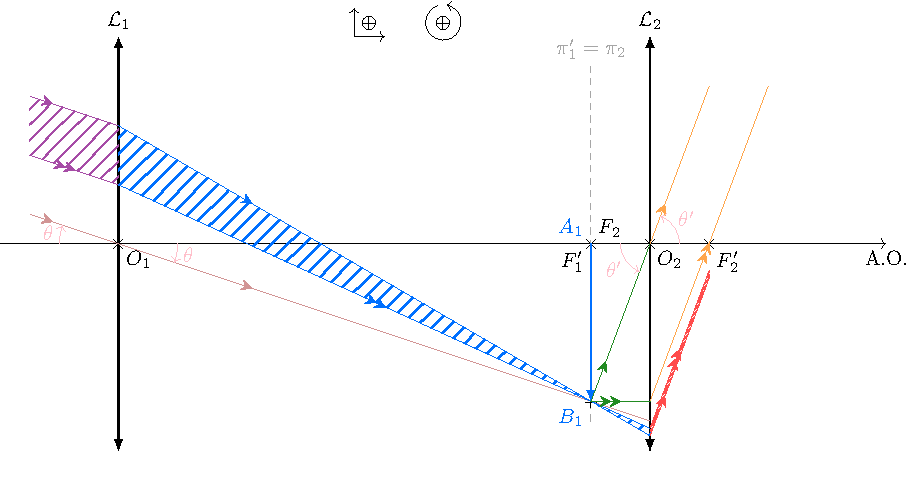
\includegraphics[width=\linewidth]{kepler.pdf}
	\end{center}

	\subsubsection{}
	\begin{tcbraster}[raster columns=6, raster equal height=rows]
		\begin{tcolorbox}[blankest, raster multicolumn=1, space to=\myspace]
			\begin{tcbraster}[raster columns=1]
				\begin{tcb}[add to natural height=\myspace, valign=top](ques)
					{Résultat}
					\[
						G
					\]
				\end{tcb}
				\begin{tcb}(tool){Outil}
					\[
						G = \frac{\theta'}{\theta}
					\]
				\end{tcb}
			\end{tcbraster}
		\end{tcolorbox}
		\begin{tcb}*[raster multicolumn=2](appl){Application}
			Avec le tracé sur le schéma et en considérant des petits angles,
			$\DS \theta' = \frac{\ABb}{\obar{O_2F_2}} > 0$ et $\DS \theta =
				\frac{\ABb}{\obar{O_1F_1'}} < 0$, soit \[ G = \frac{f_1'}{-f_2'} = -8\]
		\end{tcb}
		\begin{tcb}[raster multicolumn=3](ror)'r'{Attention}
			Pour bien voir si un angle est positif ou négatif, il faut se donner un
			sens dans lequel compter positivement, tracer les angles depuis l'axe
			optique jusqu'au rayon pour voir le changement de direction et dans la
			formule trigonométrique utiliser les grandeurs dans le bon sens.
		\end{tcb}
	\end{tcbraster}

	\subsubsection{}\label{sssec:k_cercleo}
	\begin{tcbraster}[raster columns=2, raster equal height=rows]
		\begin{tcb}(data){Cercle oculaire}
			On appelle cercle oculaire l'image de la monture de l'objectif donnée par
			l'oculaire.
		\end{tcb}
		\begin{tcb}*(inte)"left"'r'{Utilité du cercle oculaire}
			Il correspond à la section la plus étroite du faisceau sortant de
			l'oculaire, où l'œil reçoit le maximum de lumière.
		\end{tcb}
	\end{tcbraster}

	\subsubsection{}

	\begin{tcbraster}[raster columns=6, raster equal height=rows]
		\begin{tcolorbox}[blankest, raster multicolumn=3, space to=\myspacee]
			\begin{tcbraster}[raster columns=1]
				\begin{tcb}[raster multicolumn=1,
						add to natural height=\myspacee](ques){Résultat attendu}
					$$\obar{O_2C_K'}$$
				\end{tcb}
				\begin{tcb}[raster multicolumn=2](tool){Outil du cours}
					Par définition, C$_K'$ est l'image de O$_1$ par $\Lc_2$. On va
					donc se servir de la relation de conjugaison d'une lentille
					mince~:
					\[
						\frac{1}{\OFp} = \frac{1}{\OAp} - \frac{1}{\OA}
					\]
				\end{tcb}
			\end{tcbraster}
		\end{tcolorbox}
		\begin{tcb}[raster multicolumn=3](appl)'r'{Application}
			On a ici $\rm O \equiv O_2$, $\rm F' \equiv F_2'$, $\rm A \equiv O_1$ et
			$\rm A' \equiv C_K'$. On a donc~:
			\[
				\frac{1}{\obar{\rm O_2F_2'}} =
				\frac{1}{\obar{\rm O_2C_K'}} -
				\frac{1}{\obar{\rm O_2O_1}}
			\]
			et après calculs~:
			\[
				\boxed{\obar{\rm O_2C_K'} =
					\left[
						\frac{1}{\obar{\rm O_2O_1}} +
						\frac{1}{\obar{\rm O_2F_2'}}
						\right]^{-1} =
					\xul{\SI{+4.5}{cm}}
				}
			\]
		\end{tcb}
	\end{tcbraster}

	\subsubsection{}\label{sssec:k_diam}
	\begin{tcbraster}[raster columns=6, raster equal height=rows]
		\begin{tcolorbox}[blankest, raster multicolumn=3]
			\begin{tcbraster}[raster columns=1]
				\begin{tcb}[raster multicolumn=1](ques){Résultat attendu}
					\[D_K'\]
				\end{tcb}
				\begin{tcb}[raster multicolumn=2](tool){Outil du cours}
					Le diamètre du cercle oculaire s'apparente à la taille d'un
					objet. On peut donc utiliser le grandissement~:
					\[
						\g =
						\frac{\ABp}{\AB} =
						\frac{\OAp}{\OA}
					\]
				\end{tcb}
			\end{tcbraster}
		\end{tcolorbox}
		\begin{tcb}[raster multicolumn=3](appl)'r'{Application}
			Avec les données de l'énoncé, on obtient~:
			\[
				\g =
				\frac{D_K'}{D} =
				\frac{\obar{\rm O_2C_K'}}{\obar{\rm O_2O_1}}
			\]
			et finalement
			\[
				\boxed{D_K' = D\times \frac{\obar{O_2C_K'}}{\obar{O_2O_1}} =
					\xul{\SI{3.75}{mm}}
				}
			\]
		\end{tcb}
	\end{tcbraster}

	\subsection{Galilée}

	\subsubsection{}
	Si l'oculaire est divergent, cela signifie que $C_3 < 0$. On a donc $C_3 = -
		C_2$, d'où le résultat demandé.

	\subsubsection{}
	On reprend la question \ref{sssec:k_encomb}, avec cette fois des indices « 3 »
	au lieu des indices « 2 », et on obtient~:

	\begin{tcbraster}[raster columns=2, raster equal height=rows]
		\begin{tcb}(appl){Application}

			$\obar{\rm O_1O_3} = \obar{\rm O_1F_1'} + \obar{\rm F_3O_3}$
			avec
			$\obar{\rm F_3O_3} = \obar{\rm O_3F_3'} = \SI{-4}{cm}$,
			d'où
			$\xul{\obar{\rm O_1O_3} = \SI{+28}{cm}}$

		\end{tcb}
		\begin{tcb}*(inte)"left"'r'{Intérêt}
			La lunette de Galilée est donc plus compacte que la lunette de Kepler !
		\end{tcb}
	\end{tcbraster}
	\vfill
	\subsubsection{}

	\begin{center}
		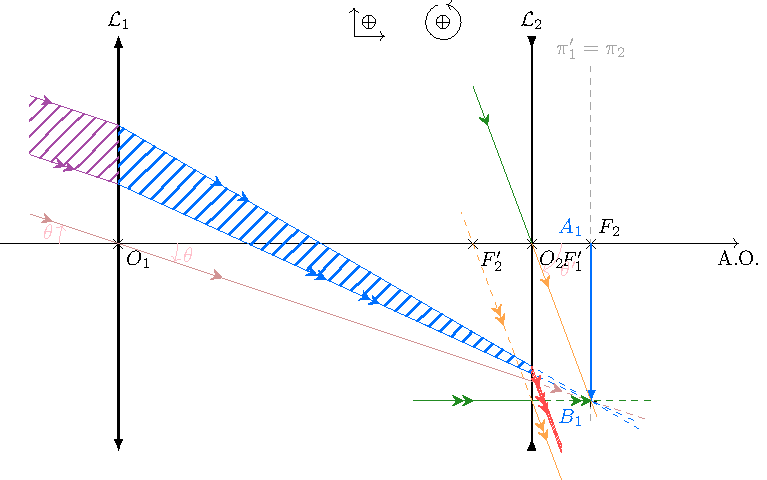
\includegraphics[width=\linewidth]{galilee.pdf}
	\end{center}

	\subsubsection{}
	On reprend la question \ref{sssec:k_cercleo}, avec des indices « 3 » au lieu de
	« 2 », et on obtient~:
	\begin{tcbraster}[raster columns=3, raster equal height=rows]
		\begin{tcb}[raster multicolumn=1](appl){Application}
			\[
				\xul{\obar{O_3C_G'} = \SI{-3.5}{cm}}
			\]
		\end{tcb}
		\begin{tcb}*[raster multicolumn=2](rema){Comparaison}
			On a cette fois un cercle oculaire virtuel. Il faudra placer son œil le
			plus près possible de l'oculaire pour espérer avoir le plus de lumière
			possible.
		\end{tcb}
	\end{tcbraster}

	\subsubsection{}
	On reprend la question \ref{sssec:k_diam}~:
	\begin{center}
		\begin{tcb}[width=.3\linewidth](appl){Application}
			\[
				\xul{D_G' = \SI{3.75}{mm}}
			\]
		\end{tcb}
	\end{center}

	\subsubsection{Comparaison}
	\begin{center}
		\begin{tabularx}{.7\linewidth}{|Y*{2}{|Y}|}\hline
			\rowcolor{gray!15}                  & Avantages                              & Inconvénients \\\hline
			\cellcolor{gray!15} Lunette Galilée & + compacte\smallbreak image droite     &
			cercle oculaire virtuel                                                                      \\\hline
			\cellcolor{gray!15} Lunette Kepler  & Grande clarté \smallbreak Cercle
			oculaire réel                       & - compacte \smallbreak image renversée                 \\\hline
		\end{tabularx}
	\end{center}
}

\end{document}
